\chapter{Weitere Beispiele f�r Dungeons und H�hlen}
\label{A_Beispiele}

Im Folgenden finden sich einige Beispiele f�r Dungeons, die mittels des Dungeongenerator-Programms generiert wurden.
Links ist jeweils die H�hle abgebildet, rechts der fertige Dungeon.
Zu jeder H�hle ist das zugrundeliegende L-System angegeben.
Anschlie�end finden sich einige Screenshots aus dem Inneren von Dungeons.

\begin{figure}[htbp]
  \centering  
  \hfill
  \subfloat{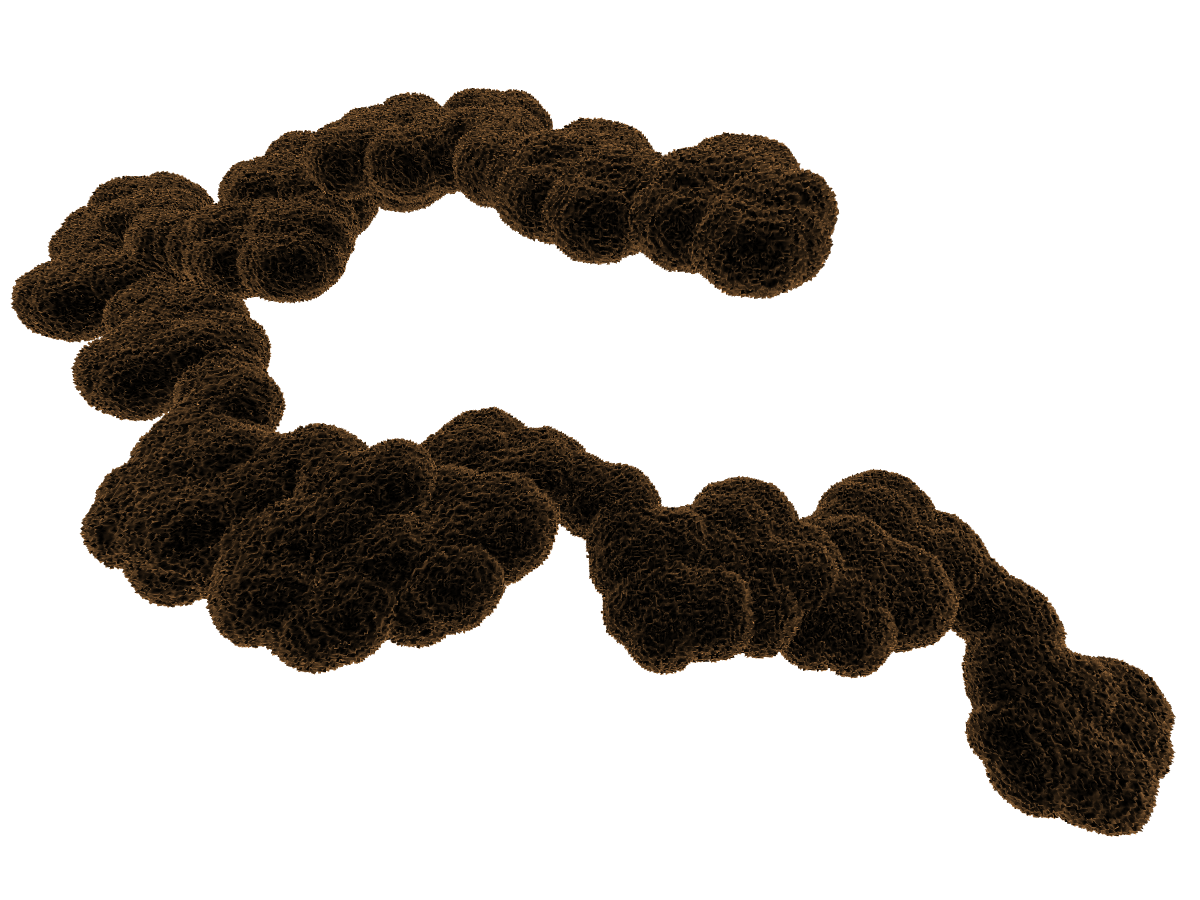
\includegraphics[width=7.4cm]{Bilder/Screenshot_Bsp_Aufsteigend_Hoehle}}
  \hfill
  \subfloat{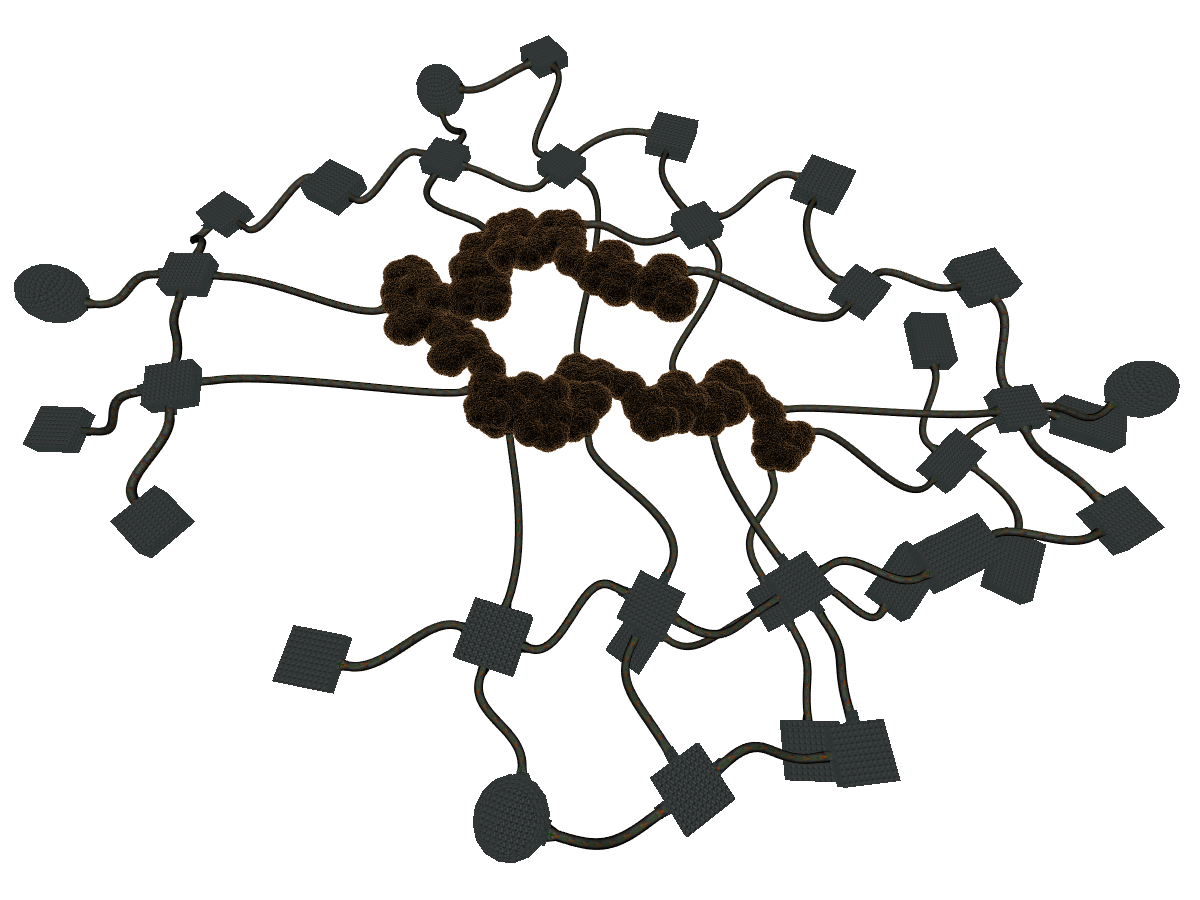
\includegraphics[width=7.4cm]{Bilder/Screenshot_Bsp_Aufsteigend_Dungeon}}  
  \hfill
	\caption[Dungeon Beispiel 1]{\emph{Dungeon Beispiel 1}:
	$G=\langle \{F,X,Y,+,-,o,\$\},YYFYF,$ \\ $
	\{
	F\rightarrow F-YX-X---,
	X\rightarrow F\$F++F-X,
	Y\rightarrow oYX--XX++
	\} \rangle$ \\
	mit $\alpha_{Gier} = 250^\circ$, $\alpha_{Nick} = 1^\circ$, Startradius $=14$, 8. Iteration
	}
	\label{B_DungeonBsp1}
\end{figure}

\begin{figure}[htbp]
  \centering  
  \hfill
  \subfloat{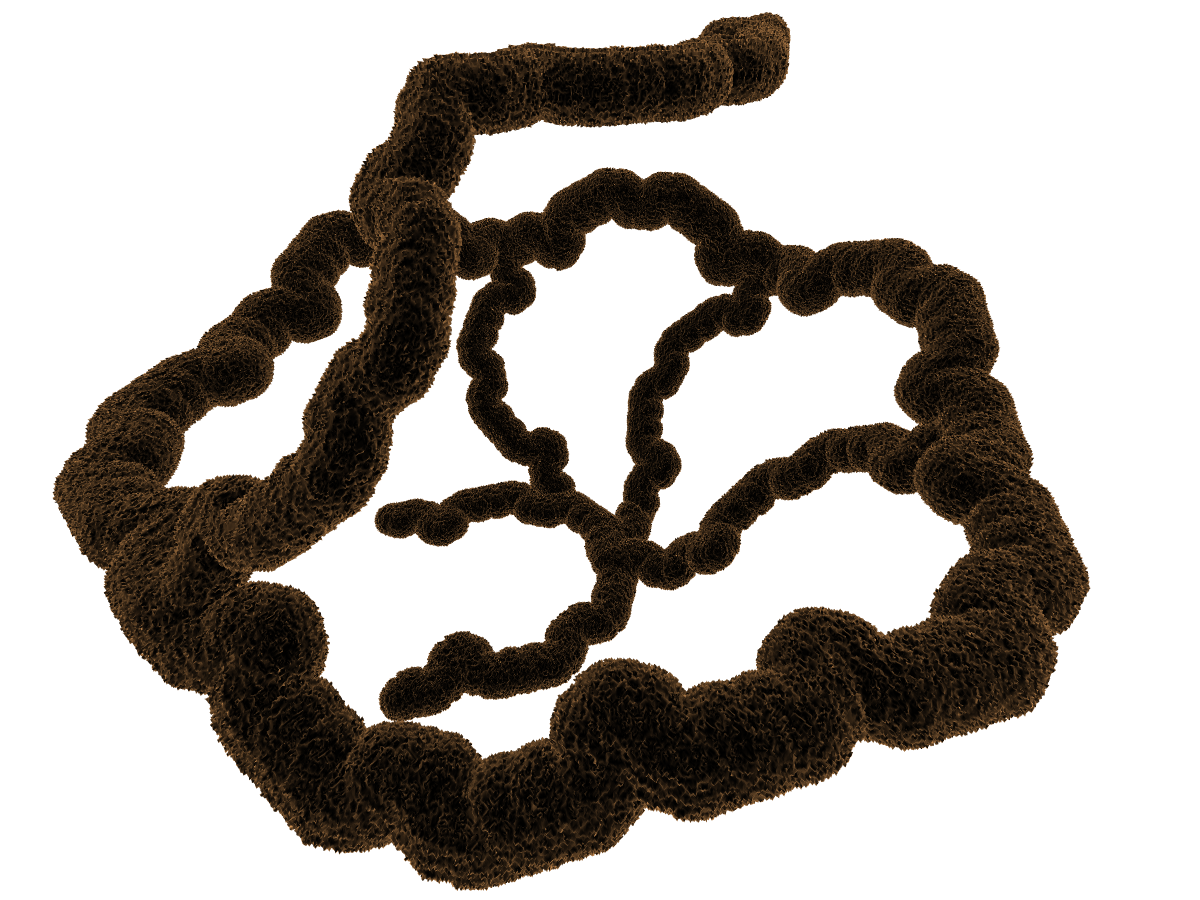
\includegraphics[width=7.4cm]{Bilder/Screenshot_Bsp_Ring_Hoehle}}
  \hfill
  \subfloat{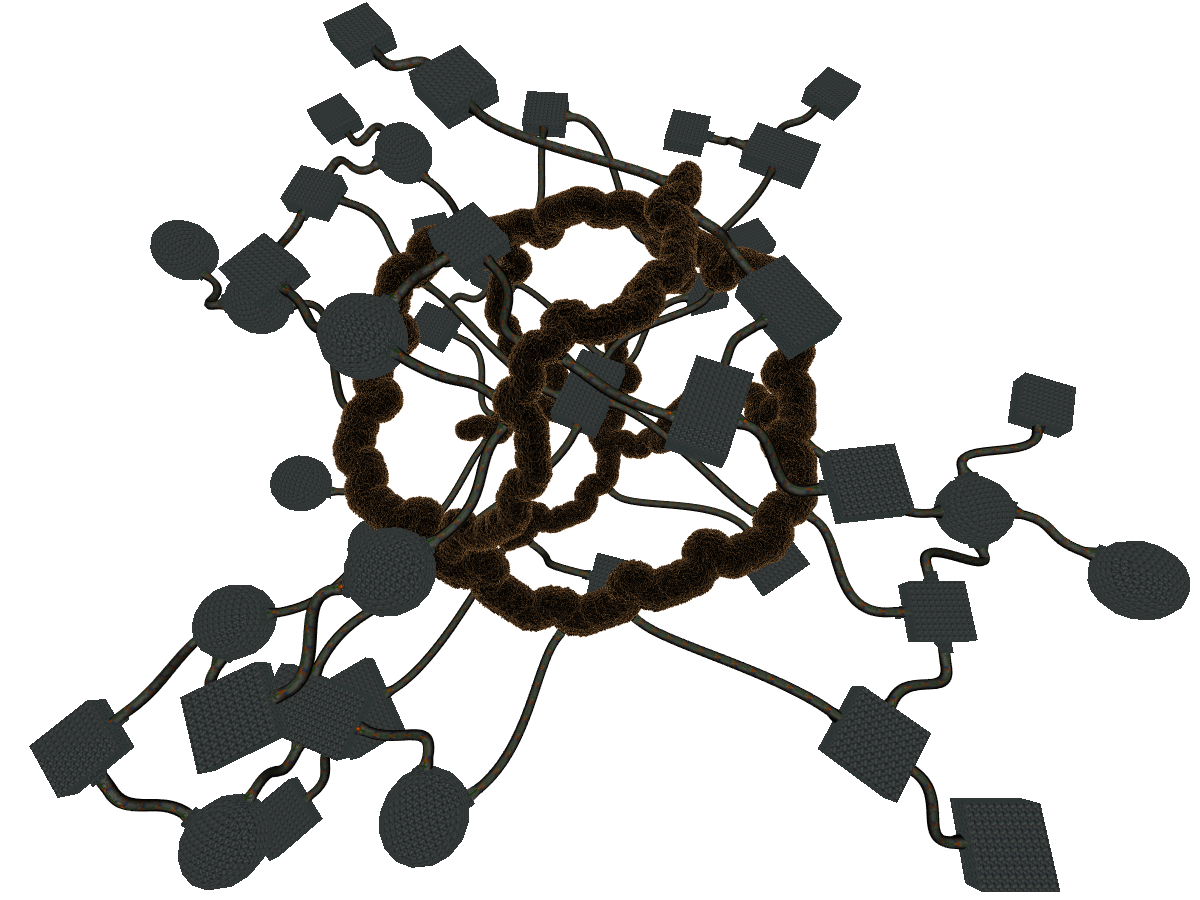
\includegraphics[width=7.4cm]{Bilder/Screenshot_Bsp_Ring_Dungeon}}  
  \hfill
  \caption[Dungeon Beispiel 2]{\emph{Dungeon Beispiel 2}:
	$G=\langle \{F,+,o,u,g,z,[,],!\},F+[!+uFoF]gFz+[!+uFozzzzF]ggFzz+[!+uF]gFz+F+[!+oFuF]zF,$ \\
	$\{F\rightarrow F-F+FF+F-F\} \rangle$ \\
	mit $\alpha_{Gier} = 60^\circ$, $\alpha_{Nick} = 45^\circ$, $\alpha_{Roll} = 20^\circ$, $r_f = 1$, $r_d = 4$, \\ Startradius $=16$, 5. Iteration
	}
	\label{B_DungeonBsp2}
\end{figure}


\begin{figure}[htbp]
  \centering  
  \hfill
  \subfloat{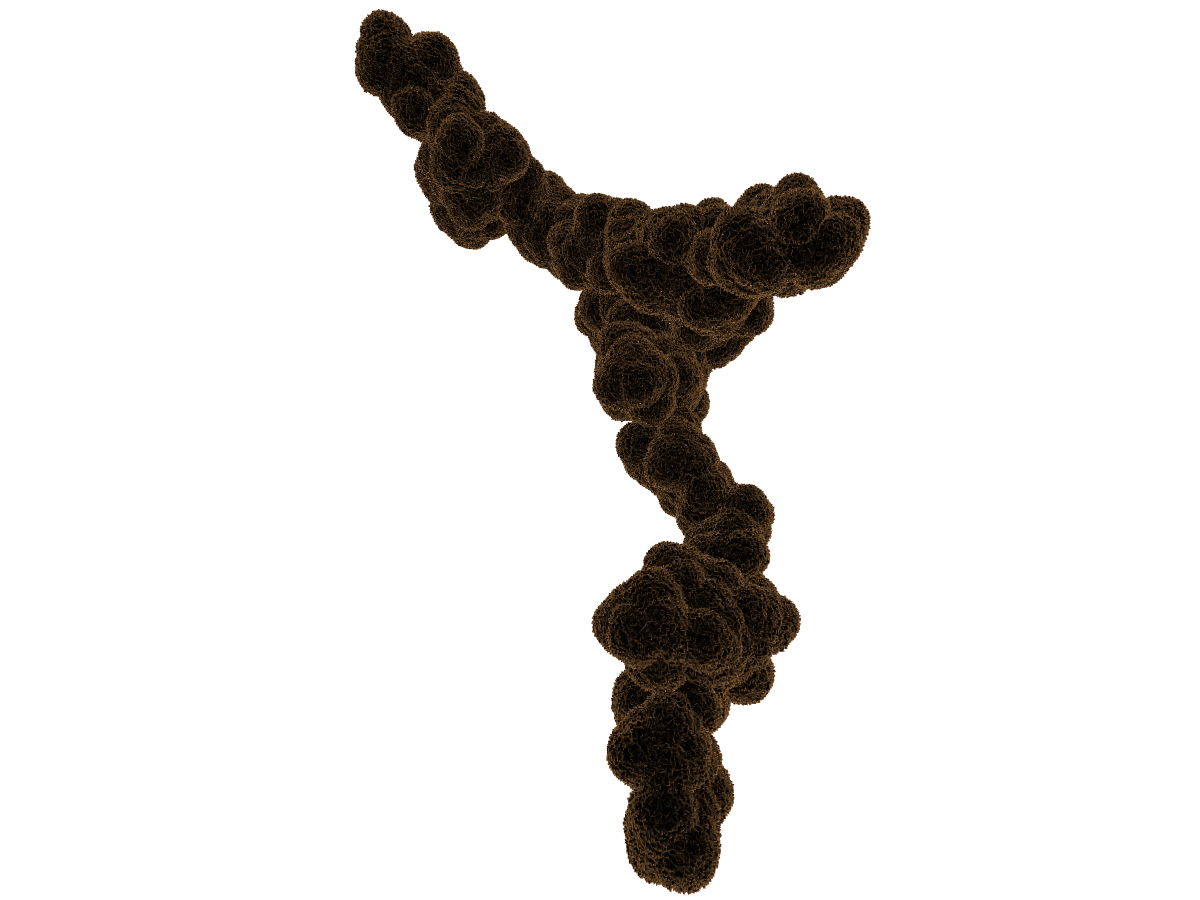
\includegraphics[width=7.2cm]{Bilder/Screenshot_Bsp_Tief_Hoehle}}
  \hfill
  \subfloat{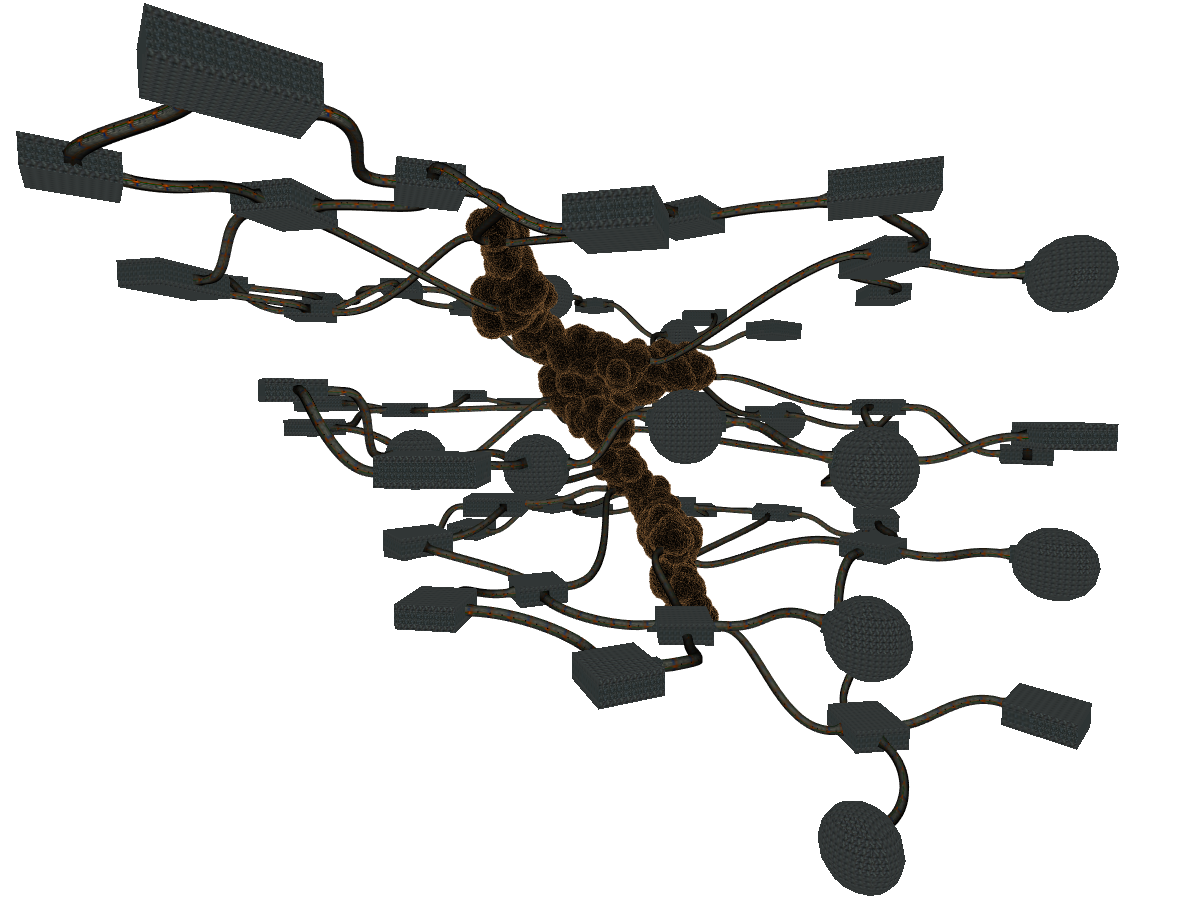
\includegraphics[width=7.2cm]{Bilder/Screenshot_Bsp_Tief_Dungeon}}
  \hfill
	\caption[Dungeon Beispiel 3]{\emph{Dungeon Beispiel 3}:
	$G=\langle \{F,+,-,o,u,g,z\},F,\{	F\rightarrow F+FoFg-FuzF\} \rangle$
	mit $\alpha_{Gier} = 285^\circ$, $\alpha_{Nick} = 255^\circ$, $\alpha_{Roll} = 255^\circ$, Startradius $=13$, 6. Iteration
	}
	\label{B_DungeonBsp3}
\end{figure}


\begin{figure}[htbp]
  \centering  
  \hfill
  \subfloat{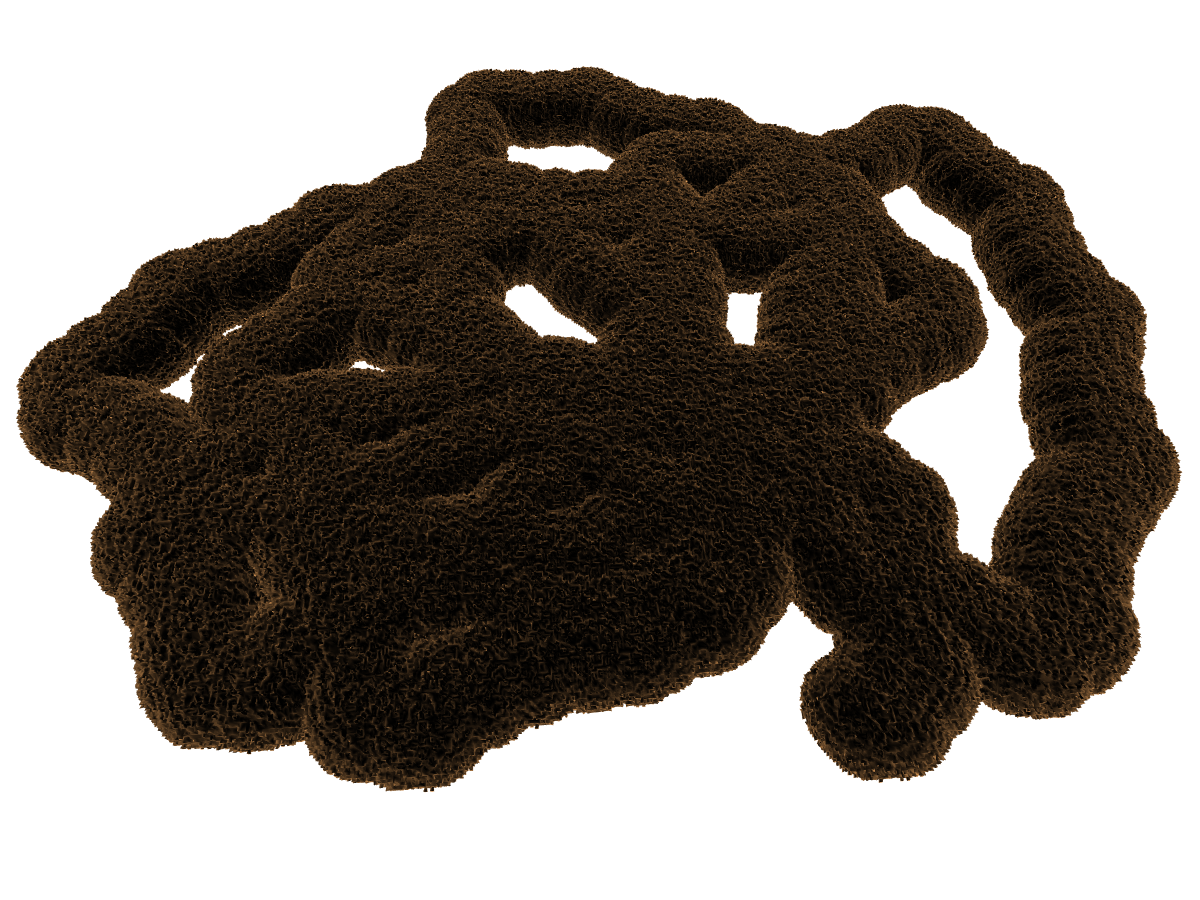
\includegraphics[width=7.2cm]{Bilder/Screenshot_Bsp_Weit_Hoehle}}
  \hfill
  \subfloat{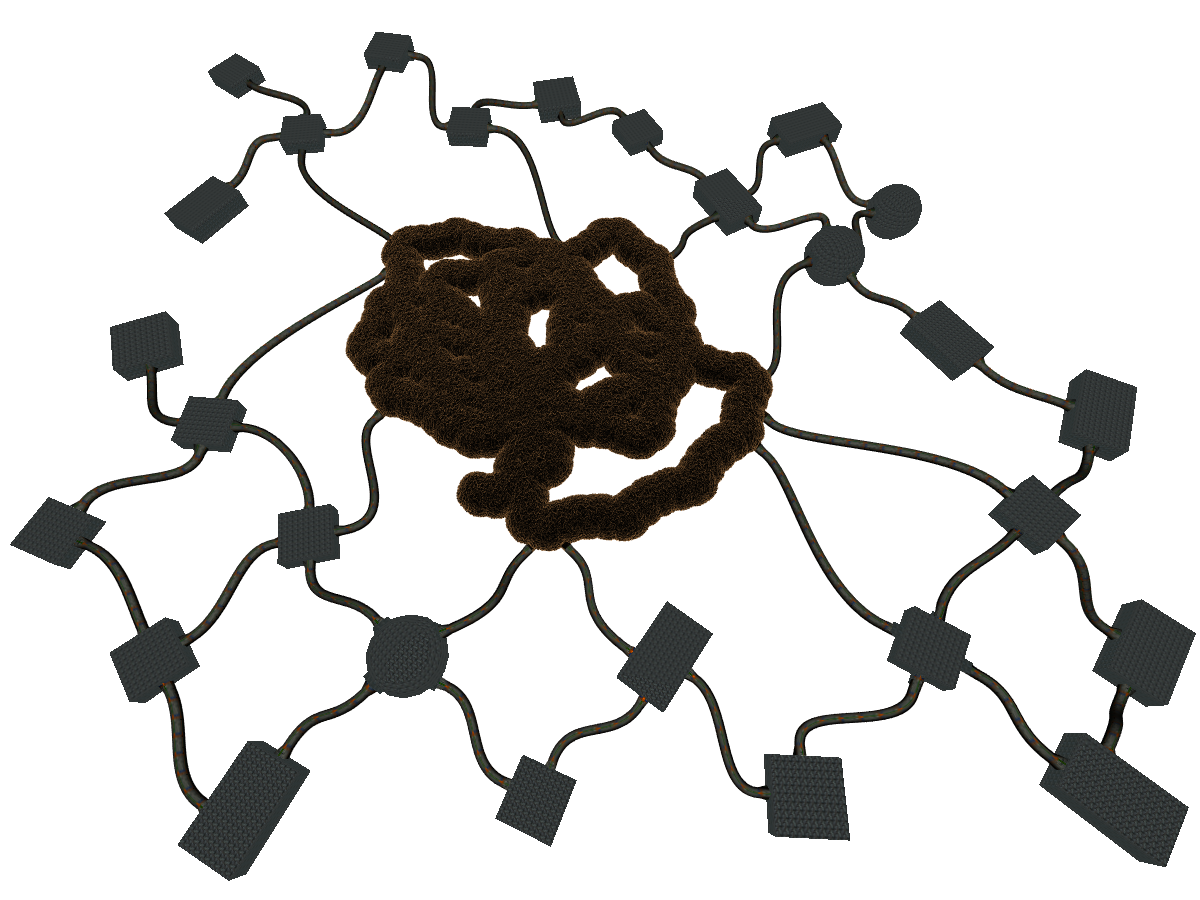
\includegraphics[width=7.2cm]{Bilder/Screenshot_Bsp_Weit_Dungeon}}  
  \hfill
	\caption[Dungeon Beispiel 4]{\emph{Dungeon Beispiel 4}:
	$G=\langle \{F,+\},F,\{F\rightarrow F+FFF\} \rangle$ \\
	mit $\alpha_{Gier} = 68^\circ$, Startradius $=16$, 7. Iteration
	}
	\label{B_DungeonBsp4}
\end{figure}

\begin{figure}[htbp]
  \centering  
  \hfill
  \subfloat{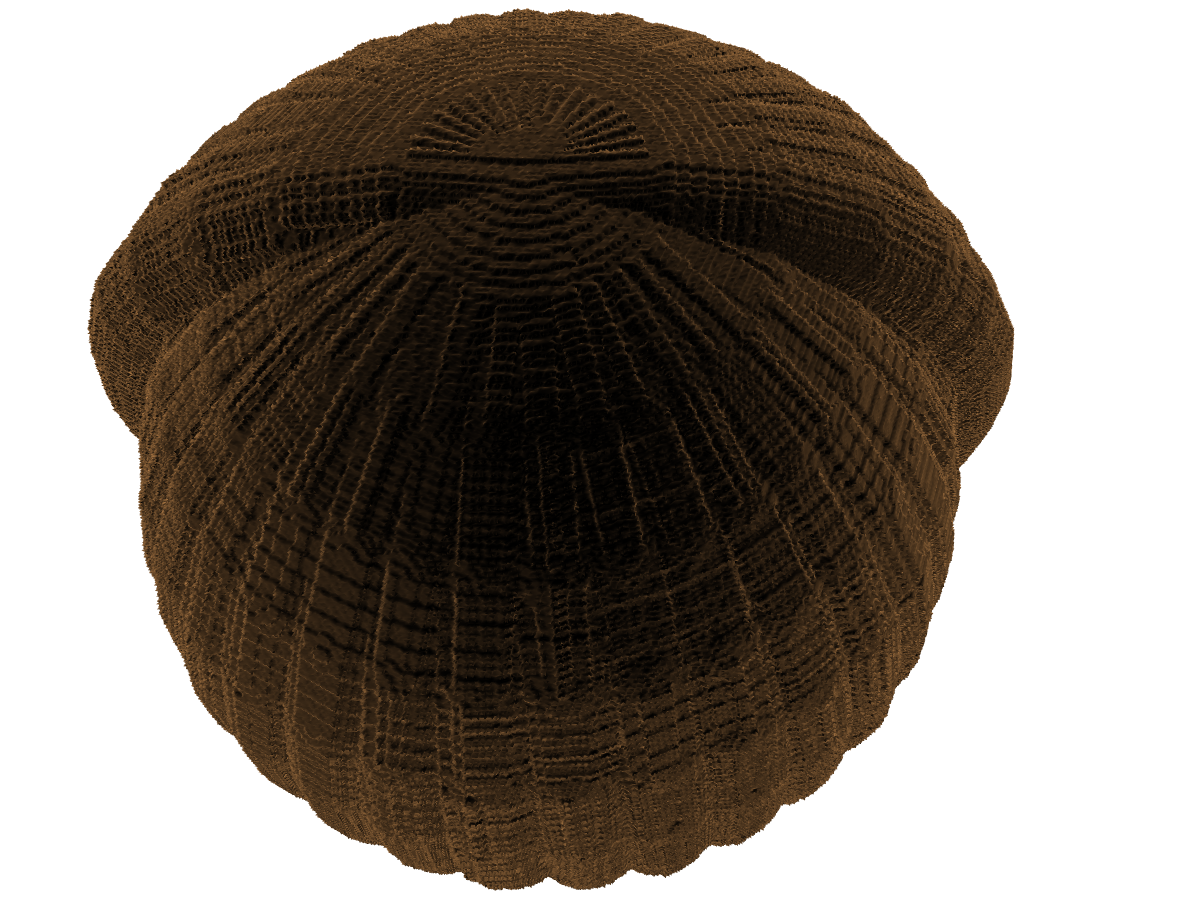
\includegraphics[width=7.2cm]{Bilder/Screenshot_Bsp_Doppelkugel_Hoehle}}
  \hfill
  \subfloat{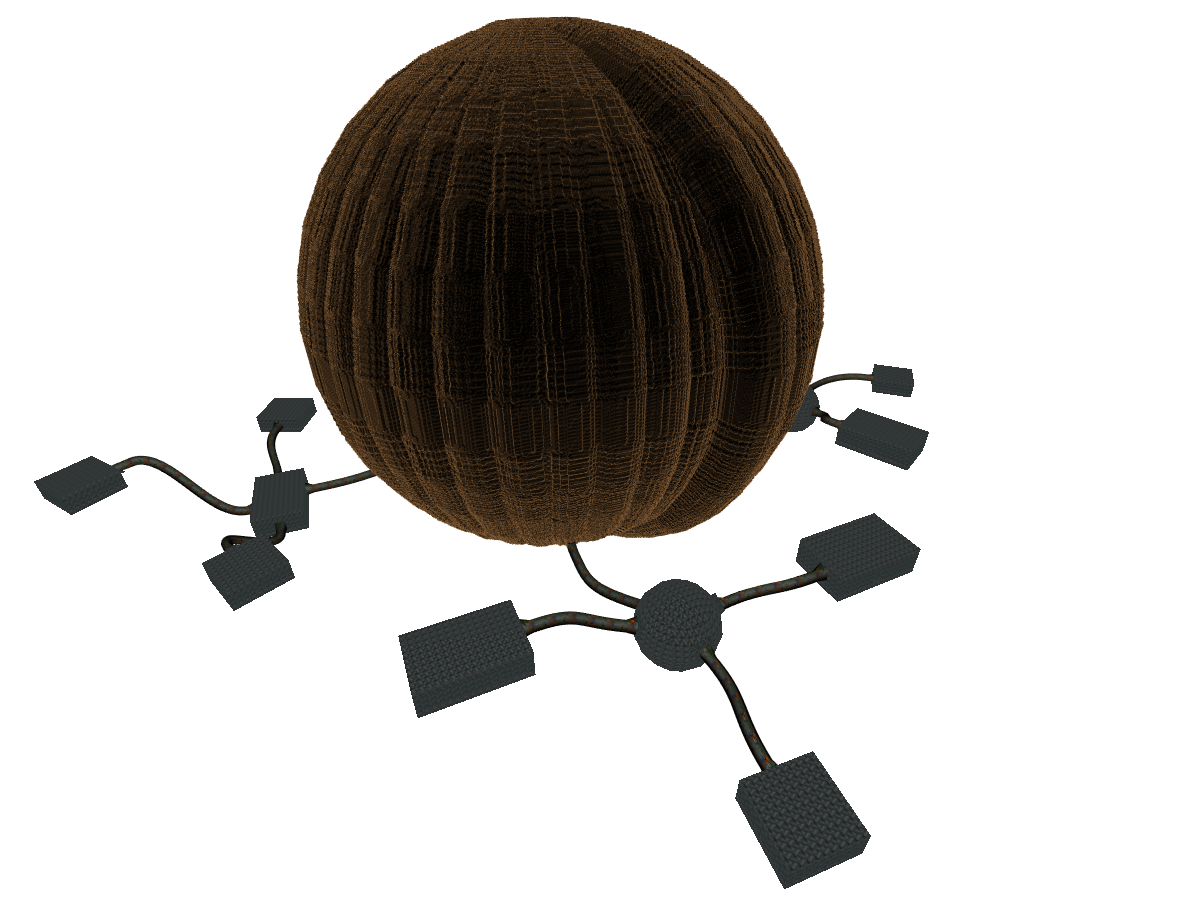
\includegraphics[width=7.2cm]{Bilder/Screenshot_Bsp_Doppelkugel_Dungeon}}  
  \hfill
	\caption[Dungeon Beispiel 5]{\emph{Dungeon Beispiel 5}:
	$G=\langle \{F,W,X,Y,+,o,[,]\},W,$ \\ $
	\{
	W\rightarrow W+[X],
	X\rightarrow YYYYYYYYY,
	Y\rightarrow FoFoFoFo
	\} \rangle$ \\
	mit $\alpha_{Gier} = 10^\circ$, $\alpha_{Nick} = 10^\circ$, Startradius $=32$, 20. Iteration
	}
	\label{B_DungeonBsp5}
\end{figure}

\begin{figure}[htbp]
  \centering  
  \subfloat{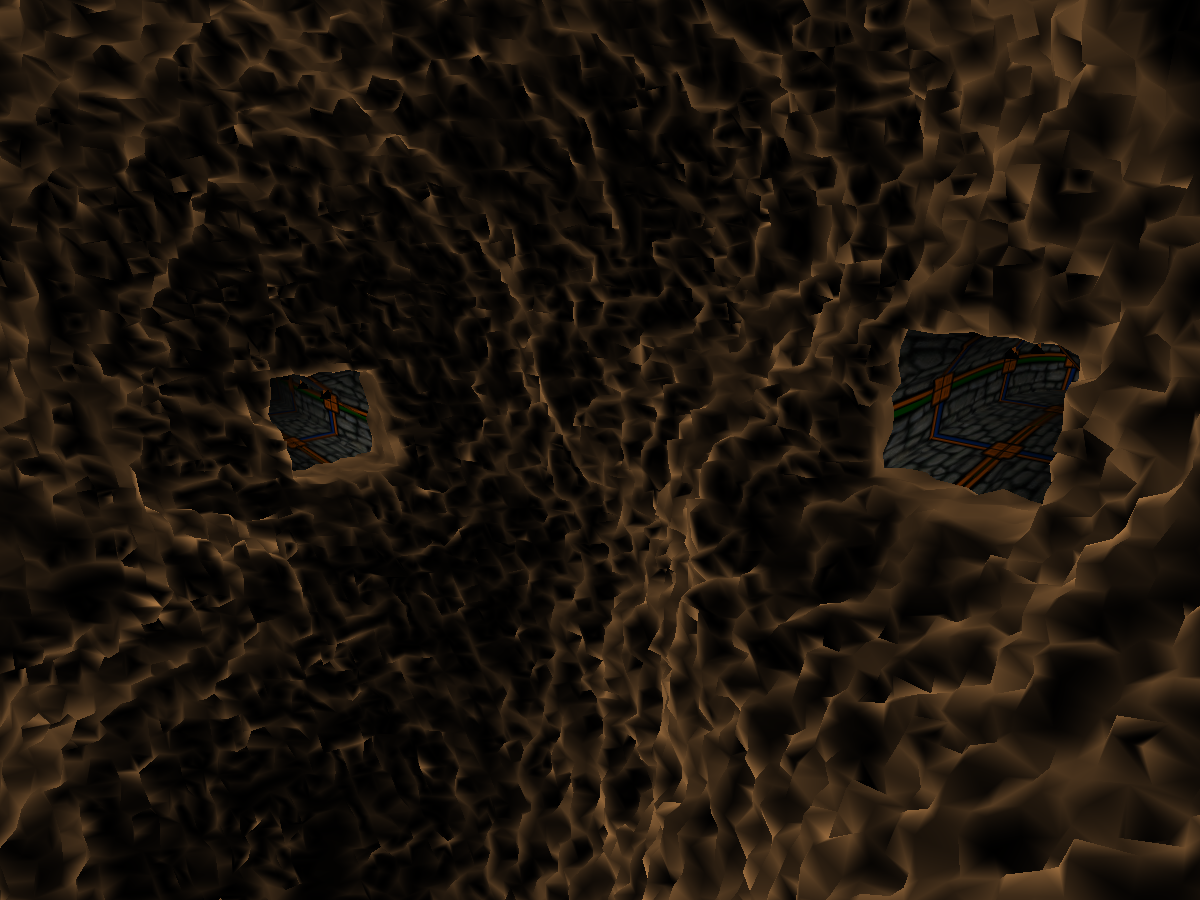
\includegraphics[width=14cm]{Bilder/Screenshot_BspShot_GaengeErosion}}\\    
  \subfloat{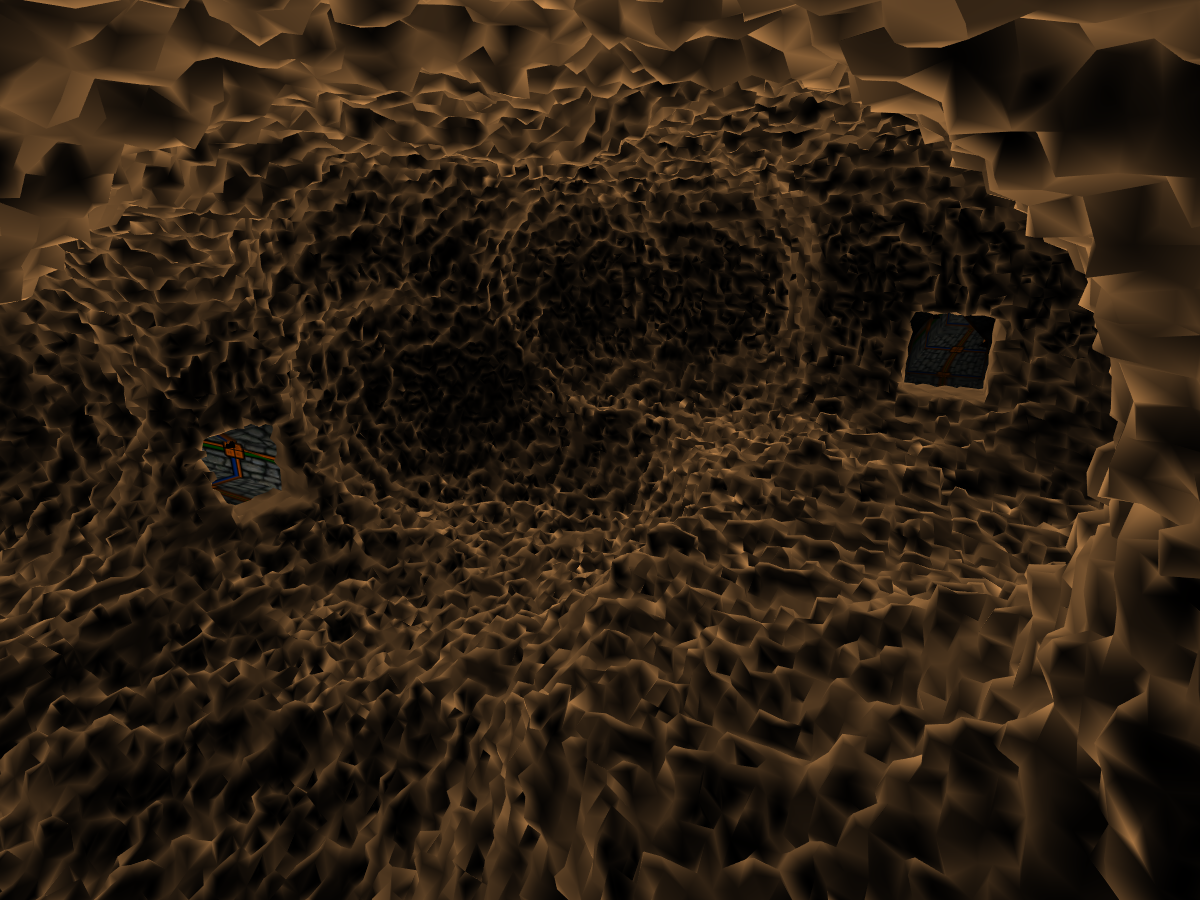
\includegraphics[width=14cm]{Bilder/Screenshot_BspShot_GaengeErosion2b}}  
	\caption[Dungeons von innen]{\emph{Dungeons von innen}: beide H�hlen unter Einfluss von Erosion, Umwandlung per Verwackeln und Gl�tten}
	 \label{B_DungeonInnenBsp1}
\end{figure}


\begin{figure}[htbp]
  \centering  
  \subfloat{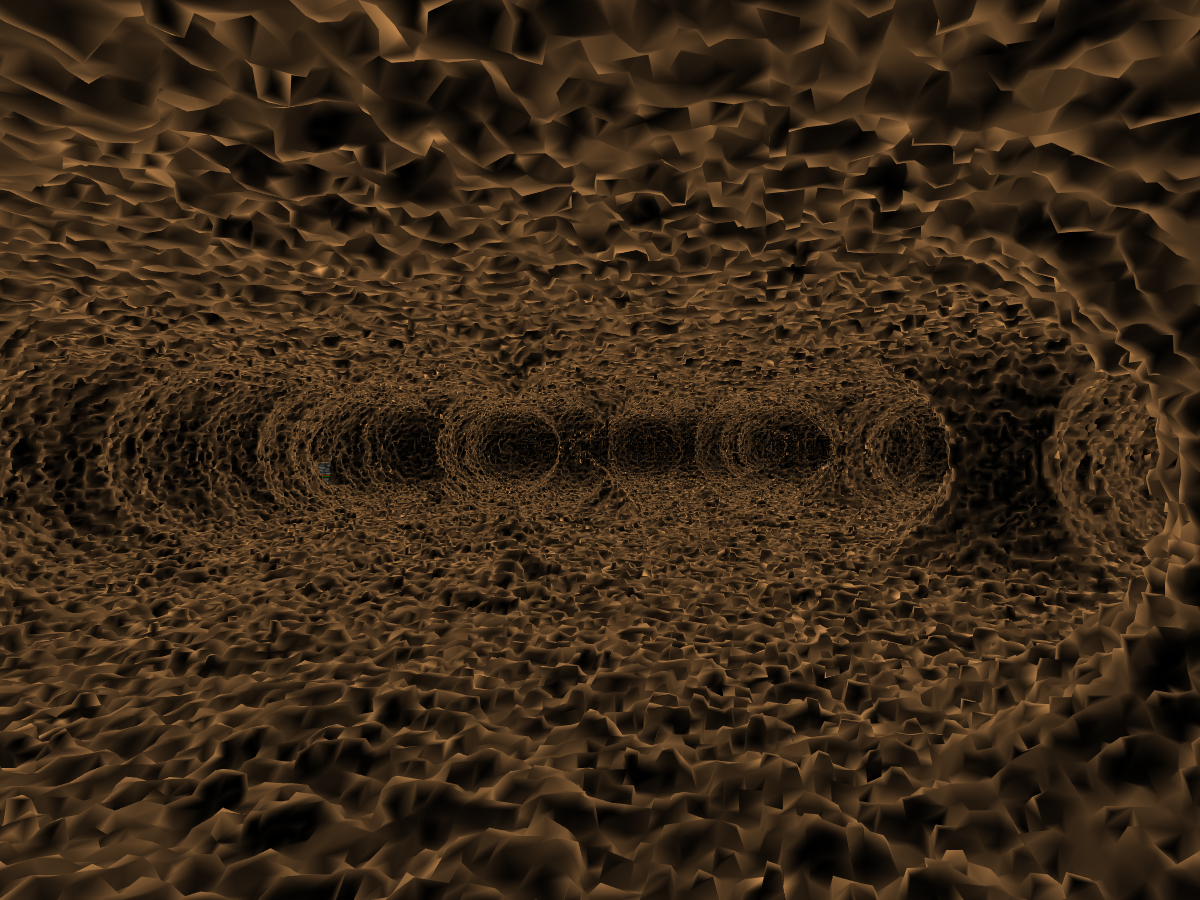
\includegraphics[width=14cm]{Bilder/Screenshot_BspShot_GaengeErosion3}}\\    
  \subfloat{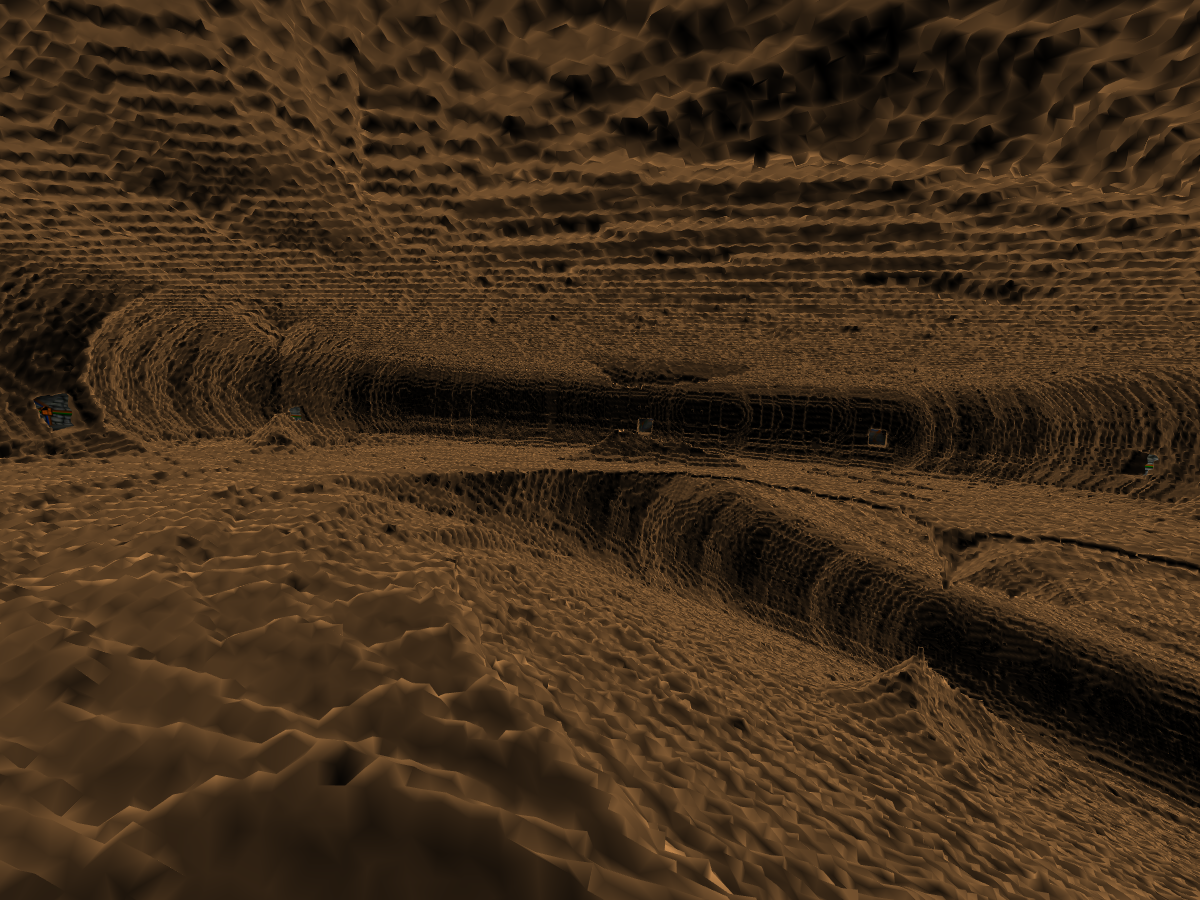
\includegraphics[width=14cm]{Bilder/Screenshot_BspShot_DungeonBizzar}}  
	\caption[Dungeons von innen ff.]{\emph{Dungeons von innen ff.} v.o.n.u. (a) H�hle unter Einfluss von Erosion, (b) H�hle ohne Einfluss von Erosion,
	beide: Verwackeln und Gl�tten}
\label{B_DungeonInnenBsp2}
\end{figure} 

